\documentclass{note}
\usepackage[table,optidef]{mypackage}

\renewcommand{\thefootnote}{\fnsymbol{footnote}}

\title{机器学习笔记}
\author{陈鸿峥}
\date{{\builddatemonth\today} \protect\footnote{\text{Build \builddate\today}}}%加了build

\begin{document}

\maketitle
\renewcommand{\thefootnote}{\arabic{footnote}}
\setcounter{footnote}{0}

\setcounter{tocdepth}{2}%设置深度
\tableofcontents

\bigskip\bigskip
本笔记对应周志华的《机器学习》(西瓜书)。

% !TEX root = main.tex

\section{计算机系统概述}
\subsection{计算模型}
\begin{itemize}
	\item 图灵机(1936)
	\item 冯诺依曼体系结构(1945)\footnote{非冯诺依曼体系结构:并行计算、量子计算、生物计算} --- 存储程序原理(\textbf{运算器}为中心)\\
	计算机采用\textbf{二进制}表示机器指令和数据,按照程序指令\textbf{顺序}执行
\begin{center}
\begin{tikzcd}
& & \text{存储器}\arrow{d} & & \\
\quad\arrow{r} & \text{输入设备}\arrow{r} & \text{运算器}\arrow{r}\arrow{d}\arrow{u} & \text{输出设备}\arrow{r} & \quad\\
& & \text{控制器}\arrow{u}\arrow{lu}\arrow{ru}\arrow[bend left]{uu} & &
\end{tikzcd}
\end{center}
而现在由于计算不是瓶颈,存储访问成为了瓶颈,故现代微机以\textbf{存储器}为中心
\begin{center}
\begin{tikzcd}
& & \text{运算器}\arrow{d} & & \\
\quad\arrow{r} & \text{输入设备}\arrow{r} & \text{存储器}\arrow{r}\arrow{d}\arrow{u} & \text{输出设备}\arrow{r} & \quad\\
& & \text{控制器}\arrow{u}\arrow{lu}\arrow{ru}\arrow[bend left]{uu} & &
\end{tikzcd}
\end{center}
\end{itemize}
[运算器、控制器](CPU)、存储器为计算机的核心,合称主机;外围设备,简称外设,指除主机外的其他设备,包括IO设备、外存等

计算机中的信息仍用二进制表示的原因:由物理器件性能决定
\begin{itemize}
	\item 二进制只有两种状态,容易找到具有2个稳定状态并且状态转换容易控制的物理器件(数字电路)
	\item 二进制编码运算规则简单
	\item 二进制的0、1与二值逻辑一致,容易实现逻辑运算
\end{itemize}
% There are two reasons computers use the binary system:
% 1.Two clearly distinct states that provide a safety range for reliability.
% 2.Least amount of necessary circuitry, which results in the least amount of space, energy consumption, and cost.

\subsection{计算机的发展历程}
按发展历程可分为:电子管、晶体管、集成电路、(超)大规模集成电路四代计算机
\par重大历史事件如下
\begin{center}
\begin{tabular}{|c|c|c|c|}
\hline
% 年份 & 姓名 & 事件 & 备注 \\
1904 & 弗莱明(Fleming) & 二极管 & \\\hline
1907 & 德福雷斯特(De Forest) & 三极管 & \\\hline
1938 & 香农(Shannon) & 布尔代数与二值电子器件(继电器) & 奠定数字电路基石 \\\hline
1946 & & 第一台通用计算机ENIAC & 十进制 \\\hline
1947 & \begin{tabular}{c}布莱顿(Brattain)\\
巴丁(Bardeen)\end{tabular} & 点接触晶体管 & \\\hline
1949 & 肖克利(Shockley) & 结型晶体管(1949) & 1956诺贝尔奖\\\hline
1950 & & 二进制和存储程序EDVAC & 实现冯诺依曼设想(组合进步) \\\hline
1958 & Jack Kilby & 集成电路 & 2000诺贝尔奖 \\\hline
1965 & Moore & 摩尔定律 & \begin{tabular}{c}
在价格不变的情况下,每18个月芯片上\\
晶体管数目翻倍,性能也提升一倍
\end{tabular}\\\hline
1971 & Intel & 第一款微处理器4004 & 10$\mu$m\\\hline
\end{tabular}
\end{center}

\subsubsection{单处理器(1971-2002)}
性能提升主要手段
\begin{itemize}
	\item 提升工作主频:KHz增长至GHz(生产工艺进步,流水线级数增加)
	\item 指令级并行(ILP)
\end{itemize}
\begin{proposition}[安迪-比尔定律]
Andy gives, Bill takes away. 安迪是原Intel CEO,比尔是原微软CEO,硬件厂商靠软件开发商用光自己提供的硬件资源得以生存
\end{proposition}
但遇到频率墙和功耗墙
\[\text{功耗(power)}\propto 1/2\times\text{CMOS电容}\times\text{电压}^2\times\text{转换(01)频率}\]
\par
2004年,Intel放弃4GHz Pentium4芯片开发,因无法解决散热问题,通过加快主频提升处理器性能的路走到尽头

\subsubsection{多核处理器(2005-)}
采用多核处理器不过是将硬件的问题丢到软件\footnote{“向多核的转变并不是因为我们在软件或体系结构技术上取得了中大突破而带来的。相反,这种转变是当单处理器体系结构发展遇到了难以克服的巨大障碍时,我们被迫作出的一种选择。”---Kurt Keutzer (UCB), \emph{The Landscape of Parallel Computing Research: A View from Berkeley}}
\begin{theorem}[阿姆达尔(Amdahl)定律]
\label{thm:amdahl}
\[\text{改进后的执行时间}=\text{受改进影响部分的执行时间}/\text{改进提高的倍数}+\text{不受影响的执行时间}\]
\[S_A=\frac{1}{s+(1-s)/N},\]
\end{theorem}
对计算机系统的某个部分采用并行优化措施后所获得的计算机性能的提高是有上限的,上限由串行部分所占的比例决定
\begin{theorem}[古斯塔夫森(Gustafson)定律]
\[S_G=(s'+p'\times N)/(s'+p')=N+(1-N)\times s',\]
其中,$s'$和$p'$为程序串行部分与可并行化部分在并行系统上执行的时间占总时间的比例,$N$为处理器数量,简便起见设总时间$s'+p'=1$
\end{theorem}
打破Amdahl定律\textbf{问题规模不变}的假设,任何足够大的任务都可以被有效地并行化,只要问题规模可扩展,并行所带来的加速比就可以扩展


\subsection{计算机系统的层次结构}
\begin{center}
\begin{tikzcd}
\text{高级语言层}\arrow{d}{}\\
\text{汇编语言层}\arrow{d}{}\\
\text{操作系统层}\arrow{d}{}\\
\text{指令系统层}\arrow{d}{}\\
\text{微体系结构层}\arrow{d}{}\\
\text{数字逻辑层}
\end{tikzcd}
\end{center}
程序编译运行过程:
\begin{center}
\begin{tikzcd}
\text{高级语言}\quad\arrow{r}{\text{预编译、编译}} & \quad\text{汇编语言}\arrow{r}{\text{汇编}} & \text{目标文件(二进制)}\arrow{r}{\text{链接}} & \text{可执行文件(二进制)}\arrow{d}{\text{加载}}\\
& & \text{电路上的电信号}\quad & \quad\text{二进制机器指令流(硬盘$\to$存储器)}\arrow[swap]{l}{\text{CPU取指译码}}
\end{tikzcd}
\end{center}
计算机内部工作过程:逐条执行加载到内存中的二进制机器指令流的过程

指令执行分为两个阶段,周期性重复性进行:
\begin{itemize}
	\item 取指阶段:CPU从内存中读取指令,程序计数器(PC)保存要被要被取出的\textbf{下一条}指令的地址,除非遇跳转指令,否则都加一个增量\footnote{程序计数器(Program Counter)是一个实际存在的寄存器吗? - Belleve的回答 - 知乎 \url{https://www.zhihu.com/question/22609253/answer/21965180} PC每次增加\textbf{一条指令的长度/寻址粒度},在MIPS中一条指令长4字节,寻址粒度1字节,故每次PC加4;而x86体系指令长度不定,每次增加量会变化}
	\item 执行阶段:对取出的指令译码后执行
\end{itemize}
软件系统可分为系统软件和应用软件

\subsection{计算机结构的八个想法}
\begin{enumerate}
	\item 摩尔(Moore)定律:集成电路资源每$18-24$个月翻倍
	\item 抽象(abstraction):简化设计
	\item 加速常用操作(Make common case fast):见定理\ref{thm:amdahl}
	\item 并行(parallelism)
	\item 流水线(pipelining)
	\item 预测(prediction)
	\item 内存等级制(hierarchy)
	\item 冗余实现可靠性(redundancy):检测故障及解决
\end{enumerate}

\subsection{基本指标}
表示计算机通信带宽时
\begin{center}
\begin{tabular}{ccccccc}\hline
KB(yte) & MB & GB & TB & PB & EB & ZB\\\hline
$10^3$ & $10^6$ & $10^9$ & $10^{12}$ & $10^{15}$ & $10^{18}$ & $10^{21}$\\\hline
\end{tabular}
\end{center}
表示计算机存储二进制时
\begin{center}
\begin{tabular}{ccccccc}\hline
KiB(yte) & MiB & GiB & TiB\\\hline
$2^{10}$ & $2^{20}$ & $2^{30}$ & $2^{40}$\\\hline
\end{tabular}
\end{center}
\begin{itemize}
	\item 位(bit/b):计算机处理、存储、传输信息的最小单位
	\item 字节(Byte/B) $1\text{ Byte}=8\text{ bit}$:现代计算机主存按字节编制,字节是最小可寻址单位
	\item 字(Word):表示被处理信息的单位,用来度量数据类型的宽度\footnote{字长是指CPU中\textbf{数据通路的宽度},等于CPU内部总线的宽度或运算器的位数或通用寄存器的宽度;字和字长的宽度可以一样,也可以不同,通常是字节的整数倍}
\end{itemize}
\par 一台32位的电脑,一个字等于4个字节,字长为32位;若字长为16位,则一个字等于2字节.
\par 4字节相当于8位16进制编码

\subsection{性能评价}
\label{subsec:performance}
CPU主频:对同一型号计算机,主频越高,完成指令一个执行步骤时间越短
\[\text{计算机的性能(Performance)}=1/\text{执行时间(Execution time)}\]
按照单位(量纲)进行换算即可
\[\begin{aligned}
\text{CPU执行时间(s)}&=\text{执行程序所需CPU时钟周期(cyc)}\times\text{时钟周期s/cyc)}\\
&=\text{指令数目(ins)}\times\text{CPI(cyc/ins)}\times\text{时钟周期(s/cyc)}
\end{aligned}\]
程序性能对执行事件的影响:
\begin{center}
\begin{tabular}{|c|c|c|c|}\hline
 & 指令数 & CPI & 时钟周期\\\hline
算法、编程语言、编译器 & $\times$ & $\times$ & \\\hline
指令集 & $\times$ & $\times$ & $\times$ \\\hline
计算机组成 & & $\times$ & $\times$ \\\hline
实现技术 & & & $\times$\\\hline
\end{tabular}
\end{center}
体系结构=指令集体系结构(功能定义与设计)+计算机组成(考虑用什么材料)\\
举例来说:
\begin{itemize}
	\item 指令集(ISA)考虑:是否提供乘法指令
	\item 组成(Organization)考虑:如何实现乘法指令(专门乘法器还是加法器+移位器)
	\item 实现技术(Technology)考虑:如何布线、用什么材料和工艺
\end{itemize}

% 带有处理器的设备一般称为智能化设备
% 完整的计算机系统应包括配套的硬件设备和软件系统
% !TEX root = main.tex

\section{基础概念}
\subsection{训练集与测试集}
\begin{itemize}
	\item 留出法(hold-out):直接将数据集划分为两个互斥的集合,一个作为训练集,另一个作为测试集
	\begin{itemize}
		\item 注意数据分布的一致性,通过多次随机划分取平均保证
		\item 通常用$2/3\thicksim 4/5$的样本用于训练,其余用作测试
	\end{itemize}
	\item 交叉验证法(cross validation)/$k$折(fold)交叉验证:划分为$k$个互斥子集,其中$k-1$个用于训练,最后一个用于验证,训练$k$次,对这$k$次结果取平均
	\begin{itemize}
		\item 通常采用10次10折交叉验证,每次都换划分方式,确保随机性
	\end{itemize}
	\item 自助法(bootstrapping):从原始数据集中放回采样得到新数据集作为测试集
	\begin{itemize}
		\item 在数据集较小的、难以有效划分训练/测试集时比较有用
		\item 但改变了初始数据集分布,会引入估计偏差
	\end{itemize}
\end{itemize}

注意:通常将习得模型实际使用中遇到的数据称为测试集,而将训练的数据划分为训练集与验证集(validation)

\subsection{参数选择}
参数通常包括
\begin{itemize}
	\item 模型本身的参数(parameter):通过学习改变
	\item 超参数(superparameter):预先设定,调参实际上就是在选择算法
\end{itemize}

\subsection{性能度量}
\begin{itemize}
\item 回归:通常采用均方误差(MSE)
\item 分类:错误率、精度
\end{itemize}

对于二分类问题,有混淆矩阵(confusion matrix)
\begin{center}
\begin{tabular}{|c|c|c|}\hline
& 预测正 & 预测反\\\hline
真实正 & TP(真正例) & FN(假反例)\\\hline
真实反 & FP(假正例) & TN(真反例)\\\hline
\end{tabular}
\end{center}
\[\begin{aligned}
\text{查准率}P&=\frac{TP}{TP+FP}\\
\text{查全率}R&=\frac{TP}{TP+FN}
\end{aligned}\]

为了衡量机器学习算法的泛化性能,需要知道以下指标:
\begin{itemize}
	\item 方差(variance):度量同样大小的训练集的变动所导致的学习性能的变化,即刻画数据扰动所造成的影响
	\[\Var{\vx}=\mathbb{E}_D\lrs{\lrp{f(\vx;D)-\bar{f}(\vx)}^2}\]
	\item 偏差(bias):度量学习算法的期望预测和真实结果的偏离程度,即刻画学习算法本身的拟合能力
	\[b^2(\vx)=\lrp{\bar{f}(\vx)-y}^2\]
	\item 噪声(noise):表达在当前任务上任何学习算法所能达到的期望泛化误差的下界
	\[\eps^2=\mathbb{E}_D\lrs{\lrp{y_D-y}^2}\]
\end{itemize}

泛化误差可以分解为
\[E(f;D)=b^2(\vx)+\Var{\vx}+\eps^2\]
即泛化性能是由学习算法的能力、数据的充分性及学习任务本身的难度决定的
\begin{figure}[H]
\centering
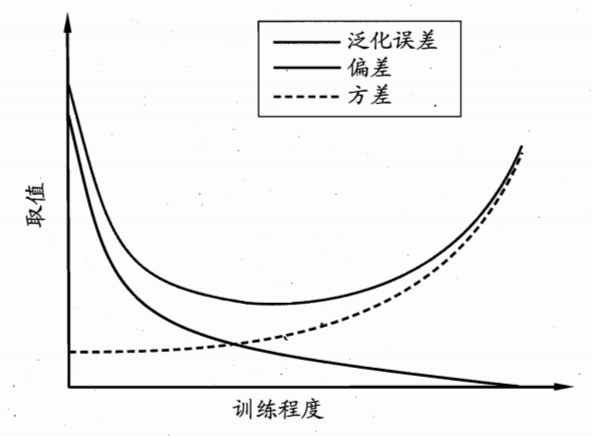
\includegraphics[width=0.4\linewidth]{fig/bias-var.png}
\end{figure}
% !TEX root = main.tex

\section{线性模型}
线性模型
\[f(\vx)=\vw^\T\vx+\vb\]
由于$\vw$直观表达了各属性在预测中的重要性,因此线性模型具有很好的可解释性(comprehensibility)。

\subsection{线性回归}
数据集$D=\{(\vx_i,y_i\}_{i=1}^m$,每个样本$\vx_i$都由$d$个属性描述,多元线性回归希望(multivariate linear regression)学到
\[f(\vx_i)=\vw^\T\vx_i+b,\;s.t.\,f(\vx_i)\simeq y_i\]

将$\vw$和$b$写在一起变成$\vw\gets\bmat{\vw & b}$,并设
\[X=\bmat{x_{11} & x_{12} & \cdots & x_{1d} & 1\\x_{21} & x_{22} & \cdots & x_{2d} & 1\\
\vdots & \vdots & \ddots & \vdots & \vdots\\x_{m1} & x_{m2} & \cdots & x_{md} & 1}=\bmat{\vx_1^\T & 1\\\vx_2^\T & 1\\\vdots & \vdots\\\vx^\T_m & 1}\]
为已知,$\vw$为需要训练的权重。
再将标记写成向量形式$\vy=\bmat{y_1 & y_2 &\cdots & y_m}$,进而得到最小二乘优化
\[\vw^\star=\argmin_\vw\norm{\vy-X\vw}_2^2\]

对$\vw$求导有
\[\nabla_\vw E_\vw=2X^\T(X\vw-\vy)\]
当$X^\T X$满秩或正定时,令上式为0有
\[\vw^\star=(X^\T X)^{-1} X^\T\vy\]
但现实中大多数时候$X^\T X$都非可逆阵,故常用正则化方法。

\subsection{线性分类}
单位阶跃(unit-step)函数
\[y=\begin{cases}
0 & z<0\\
0.5 & z=0\\
1 & z>1
\end{cases}\]
不连续,故用对数几率(logistic)函数替代
\[y=\frac{1}{1+\ee^{-z}}\]
这是一种Sigmoid函数,将线性表达式代入有
\[y=\frac{1}{1+\ee^{-(\vw^T\vx+b)}}\]
进而有
\[\vw^\T\vx+b=\ln\frac{y}{1-y}\]
将$y$视为样本$\vx$为正例的可能性,则$1-y$为反例可能性,两者比值$y/(1-y)$称为几率(odds),反映了$\vx$作为正例的相对可能性。
对数几率又称logit,故这种方法又称为逻辑斯蒂(logistic)回归,但其实是分类学习方法。

将$y$视为后验概率估计,有
\[\ln\frac{\prc{y=1}{\vx}}{\prc{y=0}{\vx}}=\vw^\T\vx+b\]
显然有
\[\begin{aligned}
\prc{y=1}{\vx}&=\frac{\ee^{\vw^\T+b}}{1+\ee^{\vw^\T\vx+b}}\\
\prc{y=0}{\vx}&=\frac{1}{1+\ee^{\vw^\T\vx+b}}
\end{aligned}\]

给定数据集$\{(\vx_i,y_i)\}_{i=1}^m$,由极大似然法估计$\vw$和$b$有
\[\ell(\vw,b)=\sum_{i=1}^m\ln\prc{y_i}{\vx_i;\,\vw,b}\]

\subsection{线性判别分析}
线性判别分析(Linear Discriminant Analysis, LDA)[Fisher, 1936]同样用于二分类,希望将样例投影到一条直线上,使得同类样例投影点尽可能近,异类样例投影点尽可能远。
\begin{figure}[H]
\centering
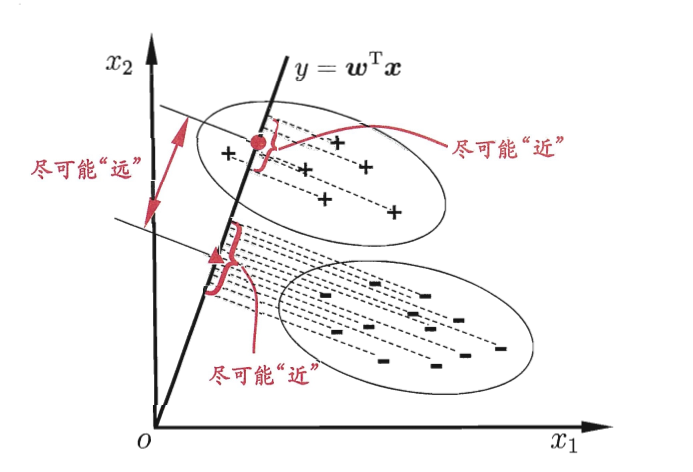
\includegraphics[width=0.5\linewidth]{fig/LDA.png}
\end{figure}

最优化广义瑞利商
\[J=\frac{\vw^\T S_b\vw}{\vw^\T S_w\vw}\]
其中$S_w$为类内散度矩阵,$S_b$为类间散度矩阵。

LDA也是经典的监督降维技术。

\subsection{类别不平衡问题}
\begin{itemize}
	\item 欠采样(undersampling):减少样例
	\item 过采样(oversampling):增加样例
	\item 阈值移动(threshold-moving)/再缩放(rescaling)
	\[\frac{y'}{1-y'}=\frac{y}{1-y}\times\frac{m^-}{m^+}\]
\end{itemize}
% !TEX root = main.tex

\section{决策树}
\subsection{信息增益}
假设当前样本$D$中第$k$类样本所占比例为$p_k$(如好瓜坏瓜二分类$M$就是$2$),则$D$的信息熵为
\[Ent(D)=-\sum_{k=1}^M p_k\log_2 p_k\]
$Ent(D)$的值越小,则$D$的纯度越高。

假设离散属性$a$有$V$个可能取值$\{a^1,a^2,\ldots,a^V\}$(如颜色属性,红蓝绿,则$a^1=R,a^2=B,a^3=G$),则产生$V$个分支结点,第$v$个结点包含取值为$a^v$的样本,记为$D^v$。
进而可以给不同分支结点赋予权值,并计算用属性$a$进行划分的信息增益(information gain)
\[Gain(D,a)=Ent(D)-\sum_{v=1}^V\frac{|D^v|}{|D|}Ent(D^v)\]
一般信息增益越大,意味着依据$a$划分所获得的纯度提升越大。
因此每次划分采用最大信息增益的属性进行划分,此即ID3(迭代二分器,Iterative Dichotomiser)决策树学习算法[Quinlan, 1986]。
\begin{figure}[H]
\centering
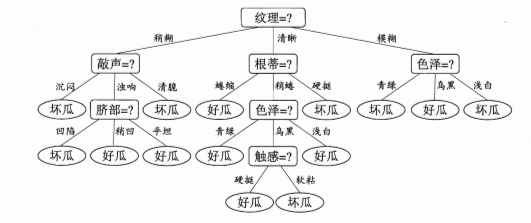
\includegraphics[width=0.6\linewidth]{fig/ID3.png}
\end{figure}

\begin{figure}[H]
\centering
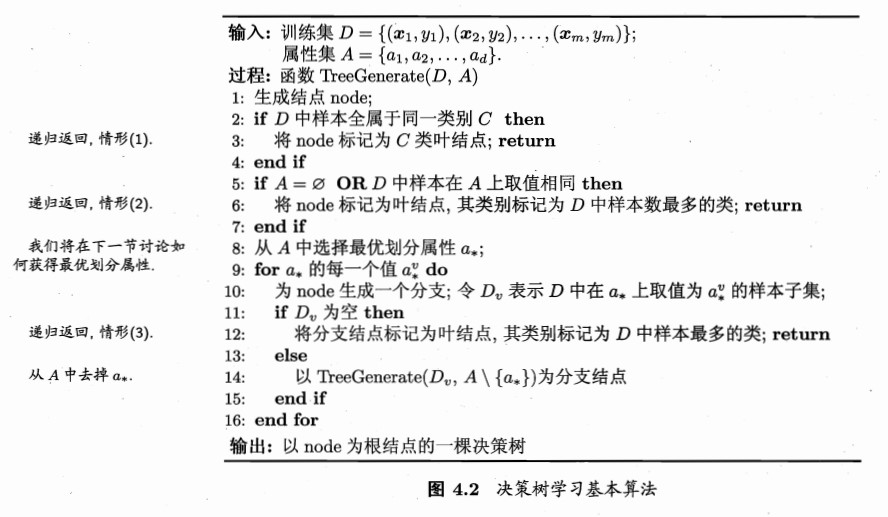
\includegraphics[width=0.8\linewidth]{fig/decision_tree.jpg}
\end{figure}

注意先前划分的指标后面可能依然会被作为划分标准,只要信息增益最大。

通过剪枝来避免过拟合
\begin{itemize}
	\item 预剪枝:对每个结点在划分前进行估计,若划分不能提升决策树泛化性能,则停止划分并将当前结点标记为叶结点,类别标记为训练样例最多的类别。
	\item 后剪枝:先完整生成一棵决策树,然后自底向上对非叶结点进行考察,若结点对应的子树替换成叶结点能够带来决策树泛化性能提升,则将该子树替换为叶结点。
\end{itemize}

类似地采用其他指标可以得到其他决策树算法:
\begin{itemize}
	\item C4.5(Classifier)算法[Quinlan ,1993]:用增益率(gain ratio)来选择最优划分属性
	\[\text{Gain\_ratio}(D,a)=\frac{\text{Gain}(D,a)}{IV(a)}\]
	其中
	\[IV(a)=-\sum_{v=1}^V\frac{|D^v|}{|D|}\log_2\frac{|D^v|}{|D|}\]
	为属性$a$的固有值(intrinsic value)。但C4.5采用启发式算法选择划分,而不是单纯基于增益率。
	\textbf{增益率准则对可取值数目较少的属性有所偏好}。
	\item CART(Classification and Regression Tree)算法[Breiman, 1984]:采用基尼指数(Gini index)
	\[\text{Gini}(D)=\sum_{k=1}^{M}\sum_{k'\ne k}p_kp_{k'}=1-\sum_{k=1}^Mp_k^2\]
	反映了从数据集$D$中随机抽取两个样本,类别标记不一致的概率。
	\[\text{Gini\_index}(D,a)=\sum_{v=1}^V\frac{|D^v|}{|D|}\text{Gini}(D^v)\]
	选择基尼指数较小的进行划分。
	CART算法包括决策树生成和决策树剪枝两个部分,回归树最小化平方误差,分类树最小化基尼指数。
\end{itemize}

理想的决策树应该是叶子结点数最少、叶子结点深度最小、叶子结点数最少且叶子结点深度最小的树。
找到这种最优的决策树是NP难题。决策树优化的目的就是要找到尽可能趋向于最优的决策树。

\subsection{连续值处理}
连续属性的离散化常用二分法,这是在C4.5算法中采用的方法。

假定连续属性$a$在$D$上出现了$n$个不同的取值,将这些值从小到大排序记为$\{a^1,a^2,\ldots,a^n\}$,基于划分点$t$可以将$D$分为子集$D_t^-$和$D_t^+$,进而可以考虑$n-1$个候选划分点集合
\[T_a=\lrb{\frac{a^i+a^{i+1}}{2}\mid 1\leq i\leq n-1}\]

\subsection{缺失值处理}
$\tilde{D}$表示$D$中在属性$a$上没有缺失值的样本子集,$\tilde{D}^v$表示$\tilde{D}$中在属性$a$上取值为$a^v$的样本子集,$\tilde{D}_k$表示$\tilde{D}$中属于第$k$类的样本子集。
为每个样本$\vx$赋予权重$w_\vx$,定义
\[\begin{aligned}
\rho &= \frac{\sum_{\vx\in\tilde{D}}w_{\vx}}{\sum_{\vx\in D}w_{\vx}}\\
\tilde{p}_k &= \frac{\sum_{\vx\in\tilde{D}_k}w_{\vx}}{\sum_{\vx\in\tilde{D}}w_{\vx}}\quad(1\leq k\leq |\mathcal{Y}|)\\
\tilde{r}_v &= \frac{\sum_{\vx\in\tilde{D}^v}w_{\vx}}{\sum_{\vx\in\tilde{D}}w_{\vx}}\quad(1\leq v\leq V)
\end{aligned}\]
分别为无缺失值样本所占的比例、无缺失样本中第$k$类所占的比例、无缺失值样本中在属性$a$上取值$a^v$的样本所占的比例。
显然有$\sum_{k=1}^{|\mathcal{Y}|}\tilde{p}_k=1$和$\sum_{v=1}^V\tilde{r}_v=1$。

可将信息增益推广为
\[\begin{aligned}
\mathrm{Gain}(D,a) &= \rho\times \mathrm{Gain}(\tilde{D},a)\\
&= \rho\times\lrp{\mathrm{Ent}\lrp{\tilde{D}}-\sum_{v=1}^V\tilde{r}_v\mathrm{Ent}\lrp{\tilde{D}^v}}
\end{aligned}\]
其中
\[\mathrm{Ent}\lrp{\tilde{D}}=-\sum_{k=1}^{|\mathcal{Y}|}\tilde{p}_k\log_2\tilde{p}_k\]

\subsection{多变量决策树}
决策树形成的分类边界有一个明显的特点,即与坐标轴平行,故学习的结果具有较好的可解释性,因为每一段划分都直接对应某个属性的取值。
但在学习任务的真实边界比较复杂时,就需要使用很多段划分才能得到比较好的近似。
\begin{figure}[H]
\centering
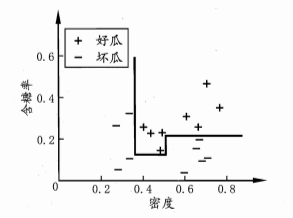
\includegraphics[width=0.4\linewidth]{fig/DT-boundary.png}
\end{figure}

如果采用线性分类器,则变成多变量决策树,可以实现更加复杂的划分。
\begin{figure}[H]
\centering
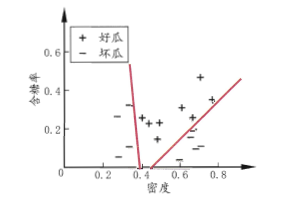
\includegraphics[width=0.4\linewidth]{fig/multivar-DT.png}
\end{figure}

决策树可能会陷入局部最优(贪心增益最高),同时分类边界表达能力弱,之后可采用随机森林的方法对性能进行提升。
% !TEX root = main.tex

\section{神经网络}
\subsection{感知机与单层神经网络}
下图是M-P神经元(neuron)模型[McCulloch and Pitts, 1943],一直沿用至今。
\begin{figure}[H]
\centering
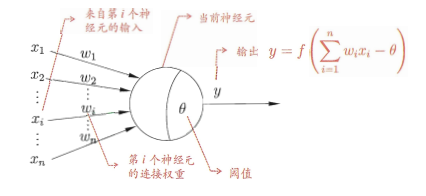
\includegraphics[width=0.6\linewidth]{fig/MP-neuron.png}
\end{figure}

感知机(perceptron)由两层神经元组成,输入层接收外界输入信号后传递给输出层,输出层是M-P神经元,亦称``阈值逻辑单元''(threshold logic unit)。
\begin{figure}[H]
\centering
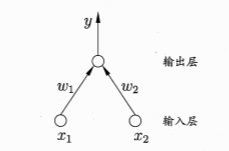
\includegraphics[width=0.4\linewidth]{fig/perceptron.png}
\end{figure}

感知机能够容易实现与或非运算,只要设定好特定的权重和阈值。

感知机的学习规则非常简单,对训练样例$(\vx,y)$,如果当前感知机的输出为$\hat{y}$,则感知机的权重依照下式修改
\[\begin{aligned}
w_i&\gets w_i+\Delta w_i\\
w_i&= \eta(y-\hat{y})x_i
\end{aligned}\]
其中$\eta\in(0,1)$称为学习率(learning rate)。
感知机预测正确则不发生变化,否则根据错误的程度对权重进行修改。

Minsky和Papert[1969]证明了若两类模式是线性可分的,则必然存在一个线性超平面将它们分开,感知机一定收敛;但非线性可分,如异或,感知机无法收敛。
\begin{figure}[H]
\centering
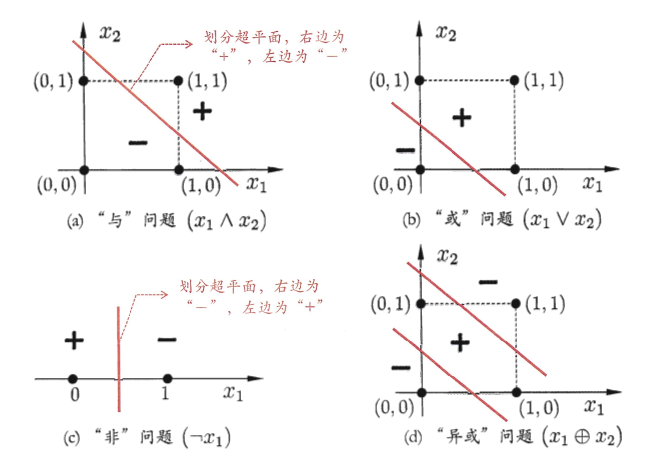
\includegraphics[width=0.7\linewidth]{fig/linear-separable.png}
\end{figure}

\subsection{多层神经网络}
要解决非线性可分问题,则需要用到多层神经网络。
\begin{figure}[H]
\centering
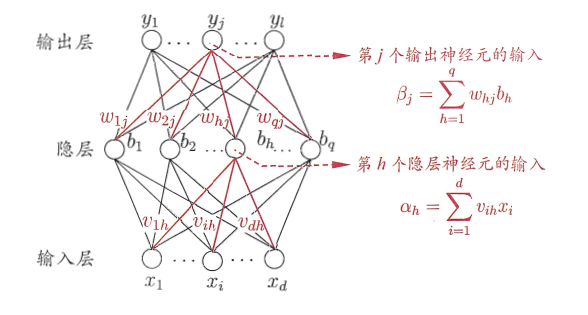
\includegraphics[width=0.6\linewidth]{fig/BP.png}
\end{figure}

用反向传播算法(Back propagation, BP)进行学习。

[Hornik, 1989]证明,只需一个包含足够多神经元的隐层,多层前馈神经网络就能以任意精度逼近任意复杂度的连续函数。
然而,如何设置神经元的个数却没有固定的标准。

\subsection{深度学习}
一般情况下,复杂模型的训练效率低,易陷入过拟合,因此难以受到人们青睐。
但是随着云计算和大数据时代的到来,计算能力的大幅提高可以有效缓解训练的低效性,训练数据的大幅增加则可以降低过拟合风险,因此以深度学习(deep learning)为代表的复杂模型开始受到人们关注。

\begin{itemize}
	\item 深度信念网络(Deep belief network, DBN)[Hinton, 2006]:每一层都是一个受限Boltzmann机
	\item 卷积神经网络(Convolutional neural network, CNN)[LeCun, 1995]:权值共享
\begin{figure}[H]
\centering
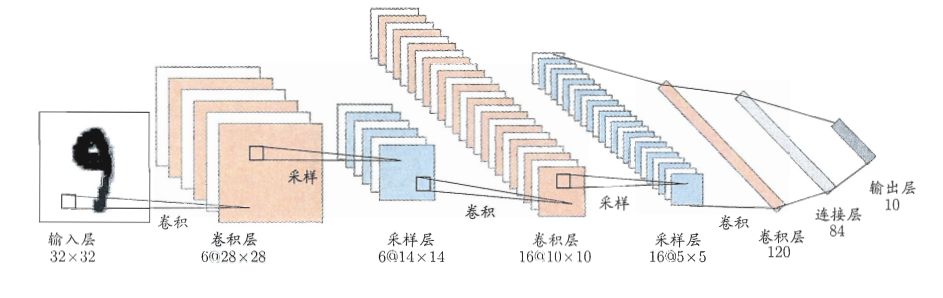
\includegraphics[width=0.8\linewidth]{fig/LeNet.png}
\end{figure}
\end{itemize}

深度学习实际上是通过多层处理,将初始的``低层''特征表示转化为``高层''特征表示后,用``简单的模型''就可以完成复杂的学习任务。(网络前若干层都是在特征表示,最后一层则是简单的分类。)
因此可以将深度学习理解为进行特征学习或表示学习(representation learning)。

以往机器学习在用于现实任务时,描述样本的特征通常需要人类专家进行设计,这称为特征工程(feature engineering)。
但现在有了深度学习,则是进一步将特征提取的工作交由机器来做。

\subsection{神经网络的历史发展}
\begin{itemize}
	\item 1940s:M-P神经元模型
	\item 1950s:感知机
	\item 1969:Minsky(MIT)出版了《感知机》一书,指出单层神经网络无法解决非线性问题,而多层神经网络训练算法看不到希望,直接导致神经网络研究进入了``冰河期''
	\item 1974:Werbos(Harvard)发明BP算法,但仍处于冰河期不受重视
	\item 1983:Hopfield(Caltech)利用神经网络在旅行商问题(TSP)上取得当时最好结果,后来Rumelhart等人重新发明BP算法,掀起神经网络第二次高潮
	\item 1990s:统计学习理论和支持向量机的兴起,神经网络学习的理论性质不够清楚、试错性强、使用中充斥大量窍门的弱点更为明显,神经网络研究又陷入低谷
	\item 2010s:算力提升+大数据涌现,神经网络在ImageNet上以绝对优势夺冠,神经网络迎来第三次高潮
\end{itemize}
% !TEX root = main.tex

\section{支持向量机}
\subsection{支持向量}
超平面由下列方程决定
\[\vw^\T\vx+b=0\]
样本空间中任意点到超平面的距离为
\[r=\frac{|\vw^\T\vx+b|}{\norm{\vw}}\]

若超平面$(\vx,b)$能将样本正确分类,则
\[\begin{cases}
\vw^\T\vx_i+b\geq +1 & y_i=+1\\
\vw^\T\vx_i+b\leq -1 & y_i=-1
\end{cases}\]
距离超平面最近的使上式成立的点称为支持向量(support vector),两个异类支持向量到超平面的距离之和为
\[\gamma=\frac{2}{\norm{\vw}}\]
被称之为间隔(margin)。
\begin{figure}[H]
\centering
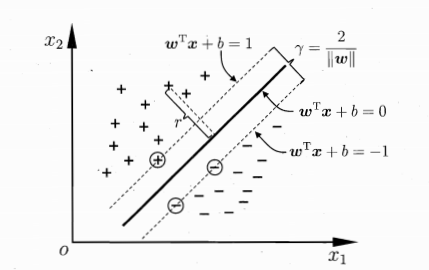
\includegraphics[width=0.6\linewidth]{fig/SVM.png}
\end{figure}

因此为找到最大间隔来划分超平面(分类结果最鲁棒,泛化能力最强),则需要求解下述最优化问题
\begin{maxi*}
{\vw,b}{\frac{2}{\norm{\vw}}}{}{}
\addConstraint{y_i(\vw^\T \vx_i+b)}{\geq 1}{\qquad i=1,2,\ldots,m}
\end{maxi*}
显然,为了最大化间隔,只需最大化$\norm{\vw}^{-1}$,等价于最小化$\norm{\vw}^2$,于是上述优化问题可重写为
\begin{maxi*}
{\vw,b}{\frac{1}{2}\norm{\vw}^2}{}{}
\addConstraint{y_i(\vw^\T \vx_i+b)}{\geq 1}{\qquad i=1,2,\ldots,m}
\end{maxi*}
此即为支持向量机(Support Vector Machine, SVM)的基本型。

可以用拉格朗日乘子法求对偶问题并得到KKT条件,可利用凸优化的方法进行求解。

对偶问题为
\begin{mini*}
{\valpha}{\frac{1}{2}\sum_{i=1}^m\sum_{j=1}^m\alpha_i\alpha_j y_iy_j\phi(\vx_i)^\T\phi(\vx_j)-\sum_{i=1}^m\alpha_i}{}{}
\addConstraint{\sum_{i=1}^m\alpha_iy_i=0}
\end{mini*}

支持向量机于[Cortes and Vapnik, 1995]正式发表,由于在文本分类任务中显示出卓越性能[Joachims, 1998],很快成为机器学习主流技术,并直接掀起统计学习(statistical learning)在2000年前后的高潮。

\subsection{核函数}
如果将非线性可分样本从原始空间映射到更高维的特征空间,则可以使其在新的特征空间中线性可分。
\begin{figure}[H]
\centering
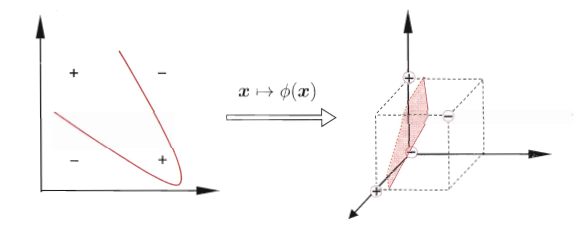
\includegraphics[width=0.6\linewidth]{fig/xor-nonlinear.png}
\end{figure}

由于$\phi(\vx_i)^\T\phi(\vx_j)$的维度可能很高,故设想有这样的核函数(kernel function)
\[\kappa(\vx_i,\vx_j)=\lrang{\phi(\vx_i),\phi(\vx_j)}=\phi(\vx_i)^\T\phi(\vx_j)\]
使得$\vx_i$和$\vx_j$在特征空间的内积等于它们在原始样本空间中通过核函数计算的结果。

几种常见的核函数如下
\begin{center}
\begin{tabular}{ccc}\hline
名称 & 表达式 & 参数\\\hline
线性核 & $\kappa(\vx_i,\vx_j)=\vx_i^\T\vx_j$ & \\
多项式核 & $\kappa(\vx_i,\vx_j)=(\vx_i^\T\vx_j)^d$ & $d\geq 1$为多项式次数\\
高斯核 & $\kappa(\vx_i,\vx_j)=\exp\lrp{-\frac{\norm{\vx_i-\vx_j}^2}{2\sigma^2}}$ & $\sigma>0$为高斯核的带宽(width)\\\hline
\end{tabular}
\end{center}

软间隔允许支持向量机在一些样本上不满足约束。
基本想法是最大化间隔的同时,让不满足约束的样本尽可能少。
\[\min_{\vw,b}\frac{1}{2}\norm{\vw}^2+C\sum_{i=1}^ml_{0/1}(y_i(\vw^\T\phi(\vx_i)+b)-1)\]
其中$l_{0/1}$是0/1损失函数
\[l_{0/1}=\begin{cases}
1 & z < 0\\
0 & \text{otherwise}
\end{cases}\]
存在的问题是0/1损失函数非凸、非连续,不易优化。

\subsection{支持向量回归}
支持向量回归(Support vector regression, SVR)允许$f(\vx)$与$y$之间最多有$\eps$的偏差
\begin{figure}[H]
\centering
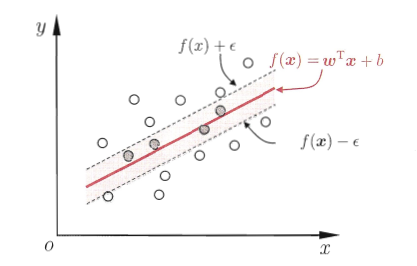
\includegraphics[width=0.6\linewidth]{fig/SVR.png}
\end{figure}

SVR问题可写为
\begin{mini*}
{\vw,b}{\frac{1}{2}\norm{\vw}^2+C\sum_{i=1}^m l_\eps(f(\vx_i)-y_i)}{}{}
\end{mini*}
其中$C$为正则化常数,$l_\eps$为$\eps$-不敏感损失($\eps$-insensitive loss)函数
\[l_\eps(z)=\begin{cases}
0 & |z|\leq \eps\\
|z|-\eps & \text{otherwise}
\end{cases}\]

\subsection{核方法}
基于核函数的学习方法统称为核方法。
最常见是通过``核化''(引入核函数),来将线性学习器扩展为非线性学习器。
% !TEX root = main.tex

\section{贝叶斯优化}
\subsection{高斯混合模型}
最常用的混合模型即高斯混合模型(Gaussian Mixture Model, GMM),
\[p(\vx)=\sum_{k=1}^K\pi_k\mathcal{N}(\vx\mid\mu_k,\Sigma_k)\]
代表有$K$个高斯分布进行混合,其中$\pi_k$为混合系数,满足
\[\sum_{k}=1^K\pi_k=1,\pi_k\geq 0,\forall k\]

求最大似然
\[\ln p(X\mid\pi,\mu,\Sigma)=\sum_{n=1}^N\ln\lrp{\sum_{k=1}^K\pi_k\mathcal{N}\lrp{\vx^{(n)}\mid\mu_k,\Sigma_k}}\]
优化变量为$\Theta=\{\pi_k,\mu_k,\Sigma_k\}$。

\subsection{EM算法}
未观测变量即隐变量(latent variable),令$X$表示已观测变量集,$Z$表示隐变量集,$\Theta$表示模型参数。
若对$\Theta$做极大似然估计,则应最大化对数似然
\[LL(\Theta\mid X,Z)=\ln P(X,Z\mid\Theta)\]
但由于$Z$是隐变量,上式无法直接求解。
这时可以通过对$Z$计算期望,来最大化已观测数据的对数边际似然(marginal likelihood)
\[LL(\Theta\mid X)=\ln P(X\mid\Theta)=\ln\sum_Z P(X,Z\mid\Theta)\]

期望最大化(Expectation-Maximization, EM)算法是常用估计参数隐变量的方法(非梯度优化)。
\begin{itemize}
	\item 期望(E)步:利用当前估计的参数值来计算对数似然的期望值
	\item 最大化(M)步:寻找能使E步产生的似然期望最大化的参数值
\end{itemize}
新得到的参数值重新被用于E步,直至收敛至局部最优解。

在GMM上用EM算法与K-means非常类似,只不过EM算法是软指派(soft assignment),而且每一个中心根据软指派数据的加权平均进行移动。b
% !TEX root = main.tex

\section{集成学习}
集成学习(ensemble learning)通过构建并结合多个学习器来完成学习任务,通常可以获得比单一学习器更为显著的泛化性能。

同质(homogeneous)集成中的个体学习器称为基学习器(base learner);而异质(heterogeneous)集成中的个体学习器则一般称为组件学习器(component learner)。
\begin{figure}[H]
\centering
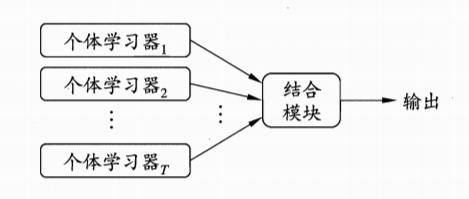
\includegraphics[width=0.5\linewidth]{fig/ensemble-learning.png}
\end{figure}

\subsection{Boosting}
提升(Boosting)可以将弱学习器提升为强学习器。

对目标函数$f(\vx)$进行多次逼近,通过不断拟合残差达到逼近的效果,可以按照下式不断迭代
\[\begin{aligned}
f_1(\vx) &=\widehat{f}(\vx)            & h_1(\vx) &=f(\vx)-f_1(\vx)\\
f_2(\vx) &=f_1(\vx)+\widehat{h_1}(\vx) & h_2(\vx) &=f(\vx)-f_2(\vx)\\
f_3(\vx) &=f_2(\vx)+\widehat{h_2}(\vx) & h_3(\vx) &=f(\vx)-f_3(\vx)\\
\vdots   &                             & \vdots \\
f_n(\vx) &=f_{n-1}(\vx)+\widehat{h_{n-1}}(\vx)
\end{aligned}\]

\subsection{Bagging与随机森林}
Bagging[Breiman, 1996]基于自助采样法,采样出$T$个含$m$个样本的采样集,然后基于每个采样集训练出一个基学习器,再将这些基学习器结合。

随机森林[Breiman, 2001]是Bagging的一个扩展变体。
传统决策树在选择划分属性时是在当前结点的属性集合(假定有$d$个属性)中选择一个最优属性;
而在随机森林中则是对基决策树的每个结点,先从该结点的属性集合中随机选择一个包含$k$个属性的子集,然后再从这个子集中选择一个最优属性进行划分。
这里的$k$即控制了随机程度,一般用$k=\log_2 d$[Breiman, 2001]。

\subsection{结合策略}
最简单的就是加权平均。

当训练数据很多时,更为强大的结合策略是使用学习法,即通过另一个学习器来进行结合。
Stacking[Wolpert, 1992]是学习法的典型代表。
这里把个体学习器称为次级学习器或元学习器(meta-learner)。

Stacking先从初始数据集中训练出初级学习器,然后生成一个新数据集用于训练次级学习器。
在新数据集中,初级学习器的输出被当作\emph{样例输入特征},而初始样本的标记仍被当作样例标记。

由于次级训练集是用初级学习器产生的,故直接用初级学习器的训练集产生次级学习器过拟合风险较大;因此常通过交叉验证或留一法,用训练初级学习器未使用的样本来产生次级学习器的训练样本。
以$k$折交叉验证为例,初始训练集$D$被随机划分为$k$个大小相似的集合$D_1,D_2,\ldots,D_k$。
令$D_j$和$\bar{D}_j=D\backslash D_j$分别表示第$j$折的测试集和训练集。
给定$T$个初级学习算法,初级学习器$h_t^{(j)}$通过在$\bar{D}_j$上使用第$t$个学习算法而得。
对于$D_j$的每个样本$\vx_i$,令$z_{it}=h_t^{(j)}(\vx_i)$,则由$\vx_i$所产生的次级训练样例的实例部分为$\vz_i=\bmat{z_{i1} & z_{i2} & \cdots & z_{iT}}$,标记部分为$y_i$。
故整个交叉验证过程结束后,从这$T$个初级学习器产生的次级训练集是$D'=\{(\vz_i,y_i\}_{i=1}^m$,然后$D'$将用于训练次级学习器。

贝叶斯模型平均(BMA)基于后验概率来为不同模型赋予权重,可视为加权平均的一种特殊实现。
% !TEX root = main.tex

\section{参考资料}
\begin{enumerate}
	\item 周志华,《机器学习》,2016
	\item Jure Leskovec, Stanford CS246: Mining Massive Data Sets, \url{http://web.stanford.edu/class/cs246/}
\end{enumerate}

\end{document}